\documentclass[12pt]{article}
\usepackage[utf8]{inputenc}
\usepackage{amsmath}
\usepackage{graphicx}
\usepackage{geometry}
\usepackage{siunitx}
\usepackage{float}
\geometry{margin=1in}
\usepackage[french]{babel}
\usepackage{listings}
\usepackage{xcolor}
\usepackage{tabularx}
\lstset{
  language=Python,
  basicstyle=\ttfamily\small,
  keywordstyle=\color{blue},
  stringstyle=\color{red},
  commentstyle=\color{gray},
  showstringspaces=false,
  breaklines=true,
  frame=single,
  extendedchars=false, % important pour que 'literate' fonctionne bien
  literate=
    {é}{{\'e}}1 {è}{{\`e}}1 {ê}{{\^e}}1 {ë}{{\"e}}1
    {à}{{\`a}}1 {â}{{\^a}}1 {ä}{{\"a}}1
    {ç}{{\c{c}}}1
    {ù}{{\`u}}1 {û}{{\^u}}1 {ü}{{\"u}}1
    {î}{{\^i}}1 {ï}{{\"i}}1
    {ô}{{\^o}}1 {ö}{{\"o}}1
}

\sisetup{output-decimal-marker = {,}, per-mode=symbol, group-separator = {\,}}

\title{Étude d'une centrale thermique solaire}
\author{Réponses aux questions}
\date{\today}

\begin{document}

\maketitle

\section*{Partie I : Étude du récepteur solaire}

\subsection*{1.1}
Les différentes raisons expliquant l'efficacité de \SI{70}{\percent} entre l'énergie solaire reçue par le récepteur et l'énergie solaire incidente sur les héliostats sont :
\begin{itemize}
  \item Réflexions imparfaites et diffusion par les miroirs ;
  \item Pertes atmosphériques (absorption et diffusion) ;
  \item Mauvais alignement ou suivi solaire imparfait ;
  \item Salissures ou vieillissement des héliostats.
\end{itemize}

\subsection*{1.2}
La puissance reçue par le récepteur depuis les miroirs est :
\begin{align*}
P_{\text{récepteur}} &= S_{\text{hel}} \cdot E_s \cdot \eta_m \\
&= \SI{75000}{m^2} \cdot \SI{1000}{W.m^{-2}} \cdot 0{,}70 \\
&= \boxed{\SI{52.5}{MW}}
\end{align*}

\subsection*{2.1}
En posant $\lambda_1=\SI{1}{\mu m}, \lambda_2=\SI{6}{\mu m}, \lambda_3=\SI{16}{\mu m}$ et $\epsilon_1=0,98, \epsilon_2 = 0,92, \epsilon_3 = 0,9, \epsilon_4 = 0,75$, on a
\begin{align*}
\epsilon(T) &= \alpha(T) \\ &= \int_{0}^{+\infty} \epsilon_{\lambda}(\lambda) f_{\lambda}(T, \lambda) \, d\lambda \\ &= \epsilon_1 \cdot F_{0-\lambda_{1} T} + \epsilon_2 \cdot (F_{0-\lambda_{2} T} - F_{0-\lambda_{1} T}) + \epsilon_3 \cdot (F_{0-\lambda_{3} T} - F_{0-\lambda_{2} T}) + \epsilon_4 \cdot (1 - F_{0-\lambda_{3} T})
\end{align*}
Pour $T=547K$ on obtient $\boxed{\epsilon=0,8890}$ et pour $T=5760$, on obtient $\boxed{\alpha=0,9628}$ (en utilisant la table de fraction d'énergie du corps noir fournie en annexe).

\subsection*{2.2}
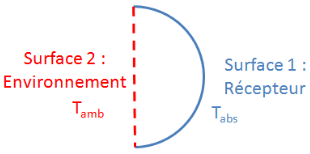
\includegraphics[scale=0.5]{img1.png} \\
Le facteur de forme \( F_{\text{e} \rightarrow \text{r}} \) de l'environnement vers le recepteur vaut trivialement 1, car l'intégralité du flux du rectangle rouge est capté. Par réciprocité :
\[
F_{\text{r} \rightarrow \text{e}} = \frac{S_e}{S_r} = \boxed{0{,}65}
\]

\subsection*{2.3}
On a :
\[
Ra = Gr \cdot Pr
\quad \text{avec} \quad 
\Delta T = \SI{254}{K},\quad L = \SI{10}{m},\quad T_m = \SI{420}{K},\quad \beta = \frac{1}{T}
\]
Aux conditions données :
\[
Pr = 0{,}7,\quad \mu = \SI{2,4e-5}{kg.m^{-1}.s^{-1}},\quad \rho = \SI{0,83}{kg.m^{-3}}, \quad \lambda = \SI{0,035}{W.m^{-1}.K^{-1}}
\]
Ainsi $Ra > 10^9$ et on utilise la corrélation :
\[
Nu_L = 0{,}13 \cdot (Gr_L \cdot Pr)^{0{,}33}
\]
Soit 
\begin{align*}
h &= 0{,}13 \cdot \frac{\lambda}{L} \cdot (Gr_L \cdot Pr)^{0{,}33} \\
&= \boxed{\SI{7,04}{W.m^{-2}.K^{-1}}}
\end{align*}

\subsection*{3.1}
La puissance absorbée après \( n \) réflexions est (démonstration par récurrence triviale):
\[
\alpha S_{\text{hel}} \eta_m E_s \cdot (\rho F_{r \rightarrow r})^n = \alpha S_{\text{hel}} \eta_m E_s \cdot \left[(1 - \alpha)(1 - F_{r \rightarrow e})\right]^n
\]
En sommant sur \( n \), on obtient :
\begin{align*}
P_{\text{abs}} &= \frac{\alpha}{1 - \alpha \cdot F_{r \rightarrow e}} \cdot S_{\text{hel}} \cdot \eta_m \cdot E_s \\
&= \frac{0{,}96}{1 - 0{,}96 \cdot 0{,}65} \cdot \SI{52.5e6}{W} \\
&= \boxed{\SI{133,89}{MW}}
\end{align*}

\subsection*{3.2}
Avec l'analogie électrique :
\[
\phi^{\text{nette}}_{r \rightarrow e} \cdot R = M^0_e - M^0_r = \sigma \left(T_a^4 - T_r^4\right)
\]
où :
\[
R = \frac{1 - \epsilon}{\epsilon S} + \frac{1}{S F_{r \rightarrow e}}
\]
D'où :
\[
\phi^{\text{nette}}_{r \rightarrow e} = \frac{\sigma S (T_a^4 - T_r^4)}{\frac{1 - \epsilon}{\epsilon} + \frac{1}{F_{r \rightarrow e}}}
\]

\subsection*{3.3}
On a :
\[
\dot{m} = \frac{\SI{66000}{kg.h^{-1}}}{\SI{3600}{s.h^{-1}}} = \SI{18.33}{kg.s^{-1}}, \quad
\Delta h = \SI{2689}{kJ.kg^{-1}} = \SI{2.689e6}{J.kg^{-1}}
\]

Ainsi la puissance transmise au fluide est:
\begin{align*}
P_{\text{fluide}} &= \dot{m} \cdot \Delta h \\ &= \SI{18.33}{kg.s^{-1}} \cdot \SI{2.689e6}{J.kg^{-1}} \\ &= \boxed{\SI{49.3}{MW}}
\end{align*}

\subsection*{3.4}
En régime permanent on a:
\[
0 = P_{abs} - \phi^{nette}_{r \rightarrow e} - P_{\text{fluide}} + \phi_{convection}
\]
Soit:
\[
P_{\text{fluide}} - P_{abs}  = -\phi^{nette}_{r \rightarrow e} + \phi_{convection}
\]

En posant
\[
A = P_{\text{fluide}} - P_{abs} \quad B = -\frac{\sigma S}{\frac{1-\epsilon}{\epsilon} + \frac{1}{F_{r \rightarrow e}}} \quad C = 2hS
\]
Cela revient à résoudre
\[
A = B(T_a^4 - T_r^4) + C(T_a - T_r)
\]
En théorie, le script python suivant qui implémente la méthode de résolution par linéarisation devrait donner la température recherchée mais l'équation n'a pas de solution, il doit y avoir une erreur quelque part.

\lstinputlisting{resolution_iterations.py}


\section*{Partie II : Dimensionnement de la pompe}

\subsection*{1}
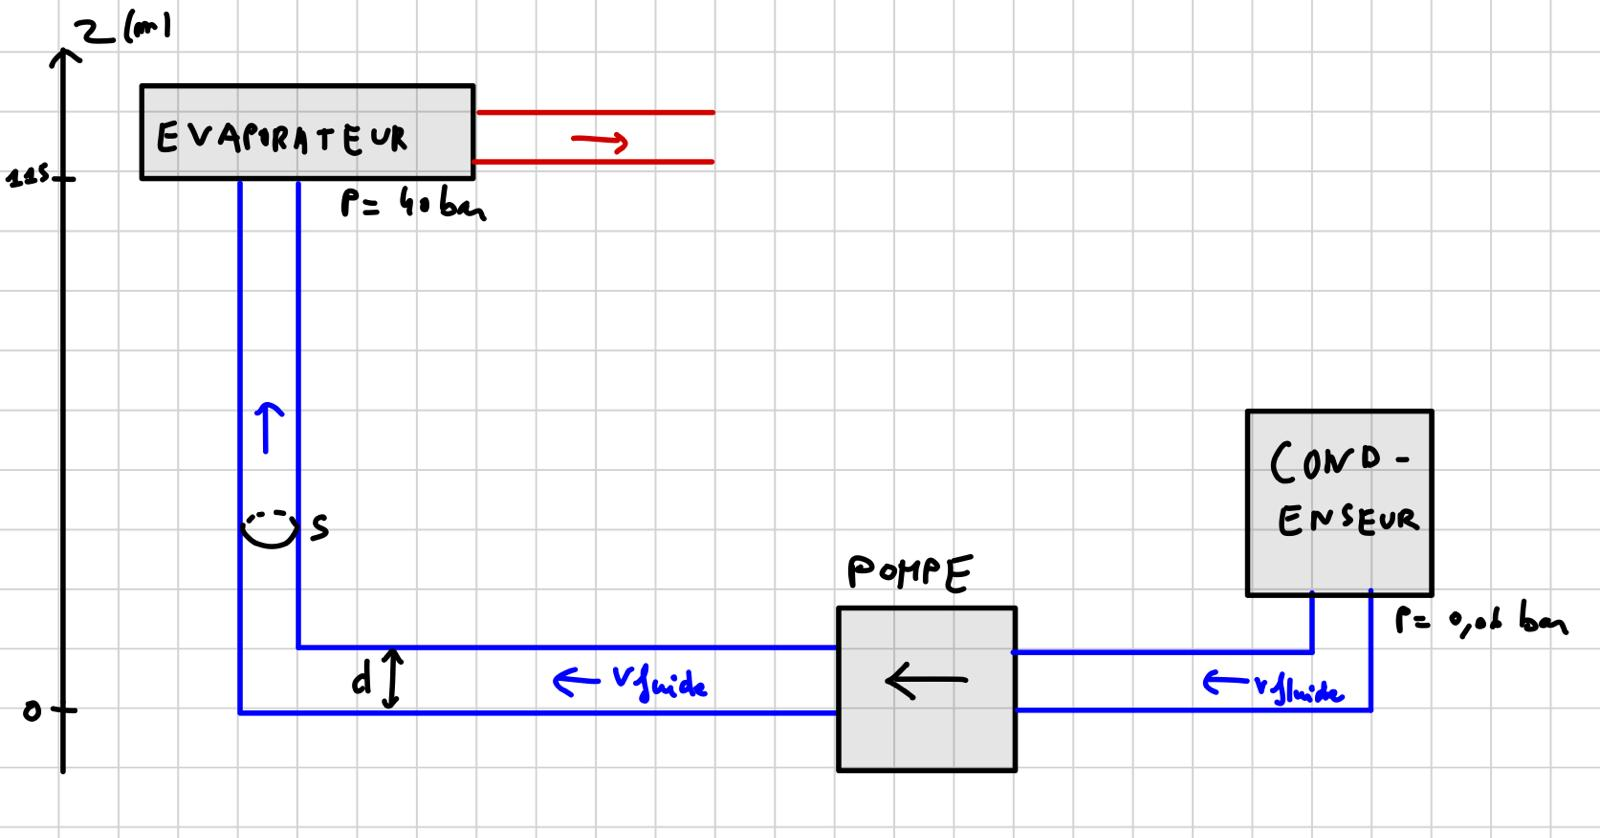
\includegraphics[scale=0.25]{2 image.jpg} \\
D'après l'énoncé on a le débit massique dans la conduite qui vaut $\dot m = 66\ 000 \ kg.h^{-1}$.

On pose la vitesse du fluide (ici un liquide) supposé constante dans toute la conduite (hypothèse à rediscuter par la suite) $v=5 \ m.s^{-1}$ pour un écoulement incompressible. En effet le fluide étant incompressible il conserve son volume, donc dans une conduite où la distribution radiale des vitesses est uniforme, il n'y a pas de raison que la conduite coudée qui part à la verticale ralentisse la vitesse du fluide, l'effet sera seulement ressenti par la pompe qui nécessitera plus de puissance.

A titre comparatif si on faisait circuler un gaz on pourrait remettre en question cette hypothèse car la gravité dans la conduite verticale pourrait compresser ce dernier et ralentir sa circulation. 

Si on commente également la vitesse du fluide de $5 \ m.s^{-1}$ on remarque qu'on reste sur un ordre de grandeur cohérent car dans les installations domestiques on ne doit pas dépasser $1$ à $2 \ m.s^{-1}$ pour des raisons de sécurité et pour limiter les pertes de charges. Ici on se place quand même sur un site de production d'énergie (dont on sait d'après les études en TD sur la centrale nucléaire, l'installation de GNL... qu'ils possèdent des installations de dimension largement supérieures à celle qu'on peut trouver la vie de tous les jours en terme de pression, taille de tuyau, température, vitesse...) ce qui justifie la multiplication par 5 tout en gardant un chiffre assez faible car on verra par la suite que les pertes de charges sont en variation quadratique par rapport à la vitesse du fluide.

A l'aide des définitions de la mécanique des fluides et les résultats concernant les fluides incompressibles on a :

$\dot m = \rho D_v = \rho S v$ où l'on note $\rho$, $D_v$ et $S$ la masse volumique ($kg.m^{-3}$), le débit volumique ($m^3.s^{-1}$) et la section de la surface ($m^2$), respectivement.

Alors $\boxed{S = \frac {\dot m}{\rho v}}$ AN : $S=3,67.10^{-3} \ m^2$.

\subsection*{2}
En notant $\eta$ la viscosité dynamique du fluide ($Pa.s$) et d le diamètre ($m$) de la conduite :

$Re=\frac{\rho v d}{\eta}$

Avec $\pi (\frac{d}{2})^2=S$ soit $\boxed{d=2 \sqrt {\frac{S}{\pi}}}$ AN : $d=0,068 \ m$.

Ainsi $\boxed{Re = \frac{2 \rho v \sqrt{S}}{\eta \sqrt{\pi}}}$ AN : $Re = 3.10^5 >> 1$.

$Re$ étant très grand, on se trouve en régime turbulent. Celui-ci homogénéise le profil de vitesse à l'intérieur du tube. En effet les pertes par frottement influencent la distribution de vitesse le long du tube, or Re caractérise le rapport entre temps caractéristique de diffusion et de convection, ici les effets d'inertie dominent. Ainsi on a une distribution de vitesse de cette forme : 

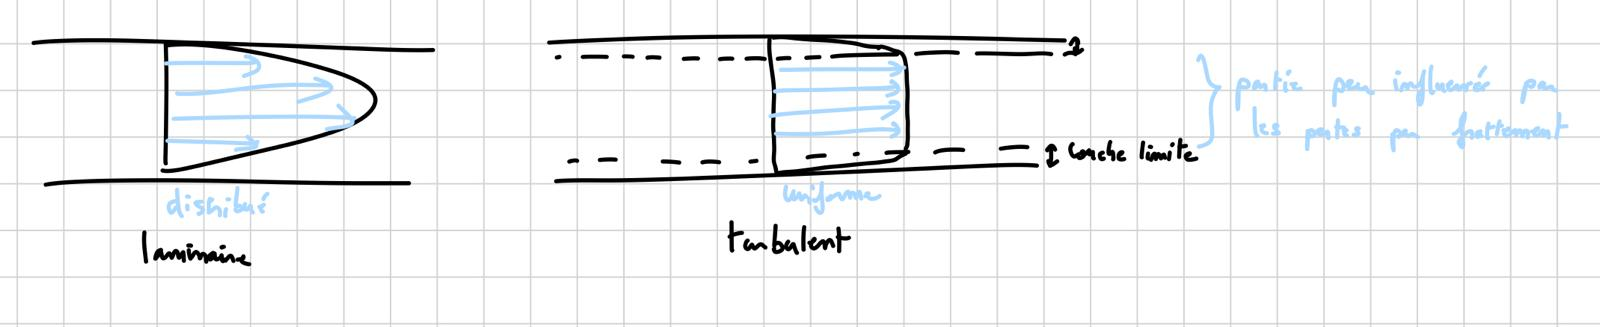
\includegraphics[scale=0.25]{1 image.jpg}

Comme on peut le voir celle-ci est uniformisée radialement. 

\subsection*{3}
Si on schématise la conduite on obtient une conduite de cette forme (schéma non orienté) :

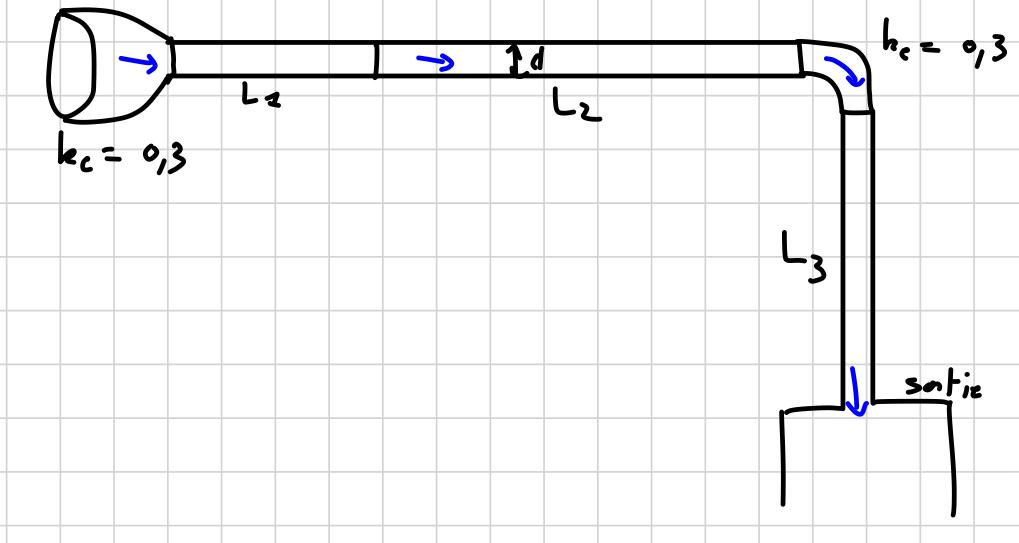
\includegraphics[scale=0.4]{3 image.jpg}

On réalise un bilan de charge de cette forme :

$\Delta \Pi = \delta E_c + \delta E_1 + \delta E_2 + \delta E_e + \delta E_3 +\delta E_s$ en correspondance avec le schéma précédent. Les passages dans la partie 1, 2, 3 sont des pertes linéiques, et les autres des pertes singulières. 

On commence par les pertes linéiques :

$\delta E_i = \lambda \frac{L_i}{d} \frac{1}{2} \rho v^2$ où on estime $\lambda$ (le coefficient de perte de charge linéique) sur le diagramme de Moody ici présent pour les valeurs 
$$
\begin{cases}
Re = 3 \cdot 10^5 \\
\frac{\varepsilon}{d} = 1{,}5 \cdot 10^{-3}
\end{cases}
$$

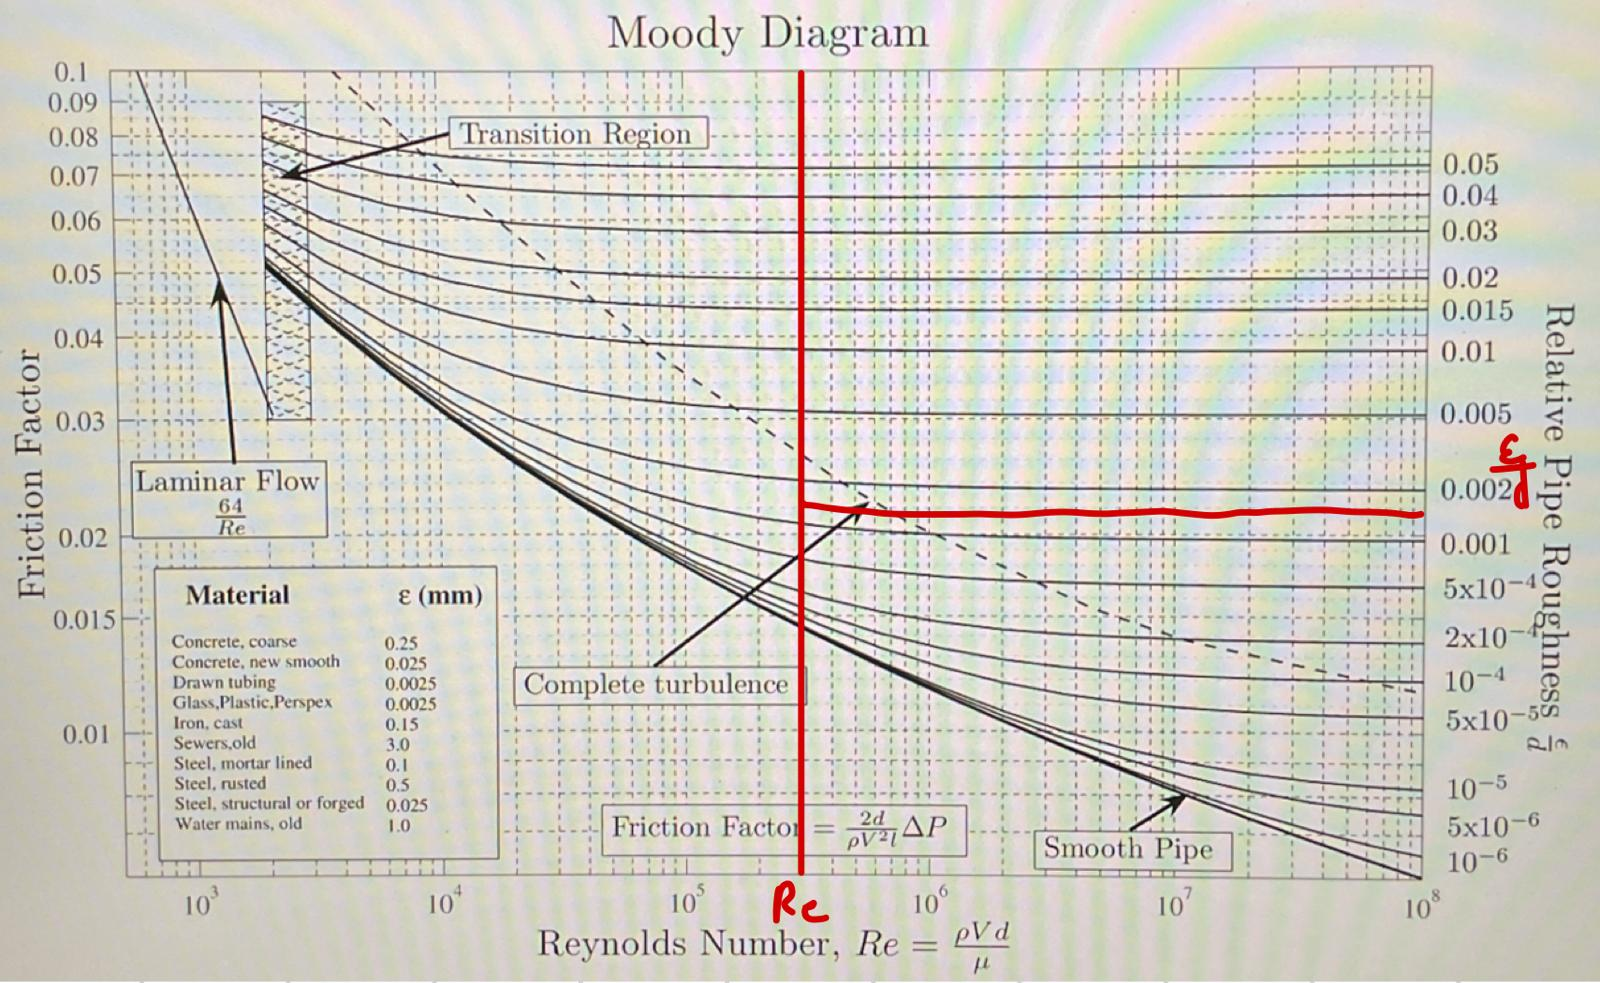
\includegraphics[scale=0.3]{4 image.jpg}

On en déduit $\lambda=0,0225$ qui vérifie la loi de Colebrook :
$$
\frac{1}{\sqrt{\lambda}} = -2 \log_{10} \left( \frac{\varepsilon}{3{,}7d} + \frac{2{,}51}{Re \sqrt{\lambda}} \right)
$$

Ensuite les pertes singulières :

$\delta E_c = k_c \frac{1}{2} \rho v^2$ d'après l'énoncé pour le coefficient de perte de charge singulière pour la bouche de captage.

$\delta E_e = k_e \frac{1}{2} \rho v^2$ pour la conduite coudée (idem)

$\delta E_s = \xi \frac{1}{2} \rho v^2 \approx (1-\frac{S_e}{S_s})^2 \frac{1}{2} \rho v^2 \approx \frac{1}{2} \rho v^2$ pour un élargissement brusque d'après les résultats du cours.

Finalement $\boxed{\delta E = [(1+k_c+k_e) + \frac{\lambda}{d}(L_1+L_2+L_3)] \frac{1}{2} \rho v^2}$ AN : $\delta E = 7,4$ bar.

\subsection*{4}
On calcule la différence de charge au long du parcours :

$\Delta \Pi_{total} = \Delta \Pi_{pompe} + \Delta \Pi_{tuyau}$

On utilise la notation E pour la partie évaporateur et C pour la partie condenseur.
On utilise la définition de la charge (qui revient à utiliser Bernoulli en quelque chose auquel on soustrait la perte de charge) :

$\boxed{\Delta \Pi_{pompe} = P_E - P_C + \rho g(z_E-z_C) - \delta E}$ AN : $\Delta \Pi_{pompe} = 43,8$ bar.

Avec un bilan d'énergie thermodynamique la puissance est de la forme $\mathcal P = \dot m \Delta h = \frac{\dot m}{\rho} \Delta P$ en notant $h$ l'entrophie et $P$ la pression.

Avec cette relation on égalise la puissance effective de la pompe qui a servi à déplacer le fluide, reliée à la perte de charge (qui s'apparente à une différence de pression) et on obtient la relation suivante $\eta \mathcal P = \Delta \Pi_{pompe} \frac{\dot m}{\rho}$.

$\boxed{\mathcal P = \frac{\Delta \Pi_{pompe} \dot m }{\eta \rho}}$ AN : $\mathcal P = 123 \ kW$.

C'est une puissance très élevée, ce qui est normal car comme évoqué à la Question 1 on se trouve dans une centrale de production énergétique de grande dimension, et il n'est pas choquant de trouver des valeurs hors du commun. En effet pour comparaison on trouve que pour une piscine classique une pompe est d'une puissance d'environ 1kW.

\section*{Partie III : Étude thermodynamique}

\textbf{Caluler les points du cycle}
\\
Nous renseignons toutes les informations sur les différents points dans le tableau suivant, les explications sont données plus bas.

\begin{table}[h!]
\centering
\begin{tabularx}{\textwidth}{|c|X|X|X|X|}
\hline
\textbf{Point} & \textbf{Température (°C)} & \textbf{Pression (bar)} & \textbf{Entropie massique (kJ/kg·K)} & \textbf{Enthalpie massique (kJ/kg)} \\
\hline
1 & 280 & 40 & 6260 & 2902 \\
\hline
2is & 50 & 0.123 & 6260 & 2004 \\
\hline
2 & 50 & 0.123 & 6950 & 2228 \\
\hline
3 & 50 & 0.123 & 704 & 209 \\
\hline
4is & - & 40 & 704 & 214 \\
\hline
4 & 50.6 & 40 & 710 & 215.25 \\
\hline
\end{tabularx}
\caption{Propriétés thermodynamiques aux 4 points du cycle}
\label{tab:points_thermo}
\end{table}

\textit{Point 1}
\\
La pression et la température sont données sur le schéma, on peut donc déduire l'entropie et l'enthalpie massique à l'aide de Coolprop.
De plus, on sait qu'il s'agit purement de vapeur à ce point là.
\\

\textit{Point 2}
\\
Pour obtenir le point 2, on détermine tout d'abord l'enthalpie du point 2is dans le cas d'une dilatation isentropique puis on utilise le rendement pour déterminer la vraie valeur de l'enthalpie ainsi que les autres informations sur ce point.
\\
La pression doit être la même qu'au point 3 (0.123 bar), et elle nous est donnée, car la transformation dans le condenseur sera isobare.
\\
Dans le domaine L+V, isobare implique isotherme donc la température sera aussi la même que le point 3, c'est à dire 50°C.
\\
En intersectant les droites verticale correspondant à une transforamtion isentropique de 1 à 2is et horizontale à une transforamtion isotherme de 2 à 3 on obtient ainsi le point 2is et donc la valeur de l'enthalpie dans le cas isentropique (voir schéma plus bas).
\\
On peut alors calculer la valeur de l'enthalpie massique du point 2 :

\begin{align*}
\eta &= \frac{\Delta h_{reel}}{\Delta h_{is}} \\
\Rightarrow h_2 &= h_1 + \eta(h_{2,is}-h_1) \\
&= 2902 + 0.75\cdot(2004-2902) \\
&= 2228 kJ/kg
\end{align*}
Une fois que l'on a ça, on peut déduire l'entropie massique à l'aide de Coolprop et on obtient 6950 kJ/kg·K.
\\

\textit{Point 3}
\\
Pour ce point, on sait qu'il se situe à 50°C et 0.123 bar sur la courbe de saturation, donc on peut déterminer toutes ses propriétés directement avec Coolprop sans faire de calculs.
\\

\textit{Point 4}
\\
On applique un raisonnement similaire à celui du point 2, mais cette fois le rendement se défini de manière inverse car c'est une pompe et non une turbine.
\\
On obtient le point 4is en intersectant la droite verticale à 704 kJ/kg·K avec l'isobare à 40 bar car la transformation 4 $\rightarrow$ 1 est isobare.
\\
On détermine ensuite le point 4 avec le calcul suivant :

\begin{align*}
\eta &= \frac{\Delta h_{is}}{\Delta h_{reel}} \\
\Rightarrow h_4 &= h_3 + \frac{h_{4,is}-h_3}{\eta} \\
&= 209 + \frac{214-209}{0.8} \\
&= 215.25 kJ/kg
\end{align*}
On peut maintenant déduire la température et l'entropie massique au point 4 pour le tracer, toujours à l'aide de Coolprop.
\\

\textbf{Les tracer dans un diagramme T-S}

insérer scan

\textbf{Calculer la puissance mécanique récupérable pour la production électrique}

\textbf{Calculer le rendement de cycle}

puissance récupérable / puissance fournie

\end{document}

